% !Mode:: "TeX:UTF-8"
% !TEX program  = xelatex

%\documentclass{cumcmthesis}
\documentclass[withoutpreface,bwprint]{cumcmthesis} %去掉封面与编号页

\usepackage{url}   % 网页链接
\usepackage{subcaption} % 子标题
\title{全国大学生数学建模竞赛编写的 \LaTeX{} 模板}
\tihao{A}
\baominghao{4321}
\schoolname{XX大学}
\membera{}
\memberb{向左}
\memberc{哈哈}
\supervisor{老师}
\yearinput{2017}
\monthinput{08}
\dayinput{22}

\title{微分方程数值解第三周第一次作业}
\begin{document}
	\maketitle
	~\\
	~\\
	
	作业:
	
	$$
	\left\{
	\begin{array}{lcl}
	-u'(x)+xu(x)=(x+1)(sinx+cosx) &, &0 \leq x \leq \pi\\
	u(0)=1,u(\pi)=-1 \\
	\end{array}
	\right.
	$$
	
	该问题的精确解为$ u(x)=sinx+cosx $.
	
	定义误差为$ E_{\infty}(h)=\max \limits_{0 \leq i \leq N}|u(x_{i}-u_i)| $.
	
	要求用紧差分格式求上述问题的数值解 求出不同步长下误差的变化,总结在步长变化时有什么规律,并通过数值例子比较中心差分格式和紧差分格式数值解的误差。
	~\\
	~\\
	解:本题的差分格式为
	\[  (-\dfrac{1}{h^{2}} +\dfrac{1}{12} x_{i-1})u_{i-1}+(\dfrac{2}{h^{2}}+\dfrac{5}{6}x_{i})u_{i}+(-\dfrac{1}{h^{2}} +\dfrac{1}{12} x_{i+1})u_{i+1}=\dfrac{1}{12}(f_{i-1}+10f_{i}+f_{i+1})\]
	
	其中,$ 1 \leq i \leq N-1 $,$ f_{i}=(x_{i}+1)(sin(x_{i})+cos(x_{i})) $,$ u_{0}=1,u_{N}=-1 $.
	
	
	
	
	
	~\\
	系数矩阵为$ Au=f $
	
	$$
	A=
	\begin{bmatrix}
	\frac{2}{h^{2}}+\frac{5}{6}x_{1}  & -\frac{1}{h^{2}}+\frac{1}{12}x_{2}  \\
	-\frac{1}{h^{2}}+\frac{1}{12}x_{1} & \frac{2}{h^{2}}+\frac{5}{6}x_{2} &-\frac{1}{h^{2}}+\frac{1}{12}x_{3} \\
	\ddots & \ddots  &  \ddots \\
	&  -\frac{1}{h^{2}}+\frac{1}{12}x_{N-2} & \frac{2}{h^{2}}+\frac{5}{6}x_{N-1}\\
	\end{bmatrix}
	$$ 
	为三对角矩阵。
	$$
	f=
	[\dfrac{1}{12}(f_{0}+10f_{1}+f_{2})+\dfrac{1}{h^{2}},\dfrac{1}{12}(f_{1}+10f_{2}+f_{3}),\cdots,\dfrac{1}{12}(f_{N-2}+10f_{N-1}+f_{N})+\dfrac{\pi}{12}-\dfrac{1}{h^{2}}]^{T}
	$$
	
	$$u=[u_{1},u_{2},\cdots,u_{N-1}]^{T}$$
	
	解题程序运行于Matlab 2018a.
	\section{数值解与精确解对比}
	
	
	步长为pi/10时的数值解与精确解对比图见图\ref{fig:duibi},误差很小,基本吻合。
	\begin{figure}
		\centering
		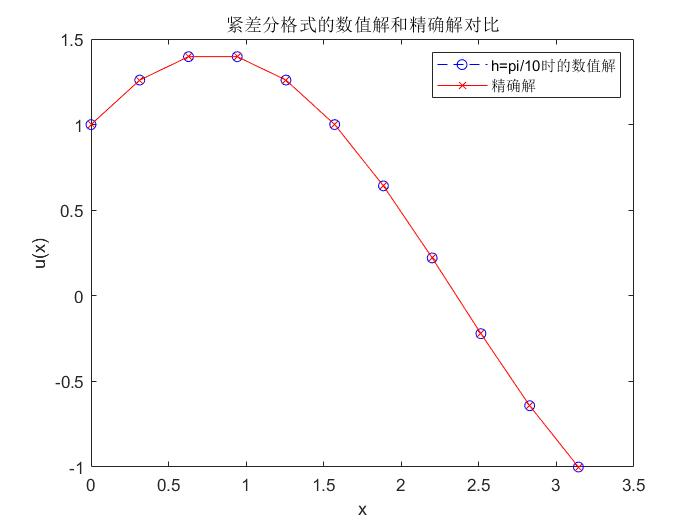
\includegraphics[width=0.7\linewidth]{figures/duibi}
		\caption{}
		\label{fig:duibi}
	\end{figure}



	
	部分节点处紧差分格式的数值解和精确解见表\ref{tab:1}。
	
	% Table generated by Excel2LaTeX from sheet '紧差分'
	\begin{table}[htbp]
		\centering
		\caption{部分节点处紧差分格式的数值解和精确解}
		\begin{tabular}{ccccc}
			\toprule[1.5pt]
			\multicolumn{1}{c}{\multirow{2}[0]{*}{h}} & \multicolumn{4}{c}{x} \\
			& \multicolumn{1}{l}{pi/5} & \multicolumn{1}{l}{2pi/5} & \multicolumn{1}{l}{3pi/5} & \multicolumn{1}{l}{4pi/5} \\
			\midrule[1pt]
			pi/10 & 1.39682105  & 1.26009409  & 0.64205189  & -0.22122884  \\
			pi/20 & 1.39680342  & 1.26007479  & 0.64204029  & -0.22123156  \\
			pi/40 & 1.39680232  & 1.26007359  & 0.64203957  & -0.22123173  \\
			pi/80 & 1.39680225  & 1.26007352  & 0.64203952  & -0.22123174  \\
			pi/160 & 1.39680225  & 1.26007351  & 0.64203952  & -0.22123174  \\
			精确解   & 1.39680225 & 1.26007351 & 0.64203952 & -0.221231742 \\
			\bottomrule[1.5pt]
		\end{tabular}%
		\label{tab:1}%
	\end{table}%
	
	部分节点处中心差分格式的数值解和精确解见表\ref{tab:2}。
	% Table generated by Excel2LaTeX from sheet '中心差分'
	\begin{table}[htbp]
		\centering
		\caption{部分节点处中心差分格式的数值解和精确解}
		\begin{tabular}{ccccc}
			\toprule[1.5pt]
			\multicolumn{1}{c}{\multirow{2}[0]{*}{h}} & \multicolumn{4}{c}{x} \\
			& \multicolumn{1}{l}{pi/5} & \multicolumn{1}{l}{2pi/5} & \multicolumn{1}{l}{3pi/5} & \multicolumn{1}{l}{4pi/5} \\
			\midrule[1pt]
			pi/10 & 1.40060902  & 1.26422701  & 0.64453215  & -0.22064412  \\
			pi/20 & 1.39775187  & 1.26111203  & 0.64266351  & -0.22108522  \\
			pi/40 & 1.39703952  & 1.26033314  & 0.64219557  & -0.22119514  \\
			pi/80 & 1.39686156  & 1.26013842  & 0.64207854  & -0.22122259  \\
			pi/160 & 1.39681707  & 1.26008974  & 0.64204928  & -0.22122945  \\
			精确解   & 1.39680225 & 1.26007351 & 0.64203952 & -0.221231742 \\
			\bottomrule[1.5pt]
		\end{tabular}%
		\label{tab:2}%
	\end{table}%
	
	由两表可知,紧差分格式比中心差分格式的数值解更加接近于精确解。
	\section{不同步长下的误差}
	紧差分格式下取不同步长时数值解的最大误差见表\ref{tab:3}。
	% Table generated by Excel2LaTeX from sheet '紧差分最大误差'
	\begin{table}[htbp]
		\centering
		\caption{紧差分格式下取不同步长时数值解的最大误差}
		\begin{tabular}{ccc}
			\toprule[1.5pt]
			\multicolumn{1}{c}{\multirow{2}[0]{*}{h}} & \multicolumn{1}{c}{\multirow{2}[0]{*}{$E_{\infty}(h)$}} & \multicolumn{1}{c}{\multirow{2}[0]{*}{$E_{\infty}(2h)/E_{\infty}(h)$}} \\
			&       &  \\
			\midrule[1pt]
			pi/10 & 2.15E-05 & \multicolumn{1}{c}{*} \\
			pi/20 & 1.34E-06 & 16.04547 \\
			pi/40 & 8.39E-08 & 15.95969 \\
			pi/80 & 5.24E-09 & 16.00292 \\
			pi/160 & 3.28E-10 & 15.99896 \\
			\bottomrule[1.5pt]
		\end{tabular}%
		\label{tab:3}%
	\end{table}%
	
	中心差分格式下取不同步长时数值解的最大误差见表\ref{tab:4}。
	% Table generated by Excel2LaTeX from sheet '中心差分最大误差'
	\begin{table}[htbp]
		\centering
		\caption{中心差分格式下取不同步长时数值解的最大误差}
		\begin{tabular}{ccc}
			\toprule[1.5pt]
			\multicolumn{1}{c}{\multirow{2}[0]{*}{h}} & \multicolumn{1}{c}{\multirow{2}[0]{*}{$E_{\infty}(h)$}} & \multicolumn{1}{c}{\multirow{2}[0]{*}{$E_{\infty}(2h)/E_{\infty}(h)$}} \\
			&       &  \\
			\midrule[1pt]
			pi/10 & 4.3432E-03 & \multicolumn{1}{c}{*} \\
			pi/20 & 1.0848E-03 & 4.0036  \\
			pi/40 & 2.7201E-04 & 3.9881  \\
			pi/80 & 6.8000E-05 & 4.0002  \\
			pi/160 & 1.7002E-05 & 3.9995  \\
			\bottomrule[1.5pt]
		\end{tabular}%
		\label{tab:4}%
	\end{table}%
	
	可知紧差分格式的数值解的最大误差小于中心差分格式,步长变为原来的$ \dfrac{1}{2} $,紧差分格式的最大误差为原来的$ \dfrac{1}{16} $,
	中心差分格式的最大误差为原来的$ \dfrac{1}{4} $,
	这是因为紧差分格式的截断误差为$ O(h^{4}) $,中心差分格式的截断误差为$ O(h^{2})$。
	
	绘制不同步长下的紧差分格式数值解的误差见图\ref{fig:wucha},步长越小,误差越小,且同一步长的误差都随着x的增大先增大后减小,在x=1左右达到最大。
	\begin{figure}
		\centering
		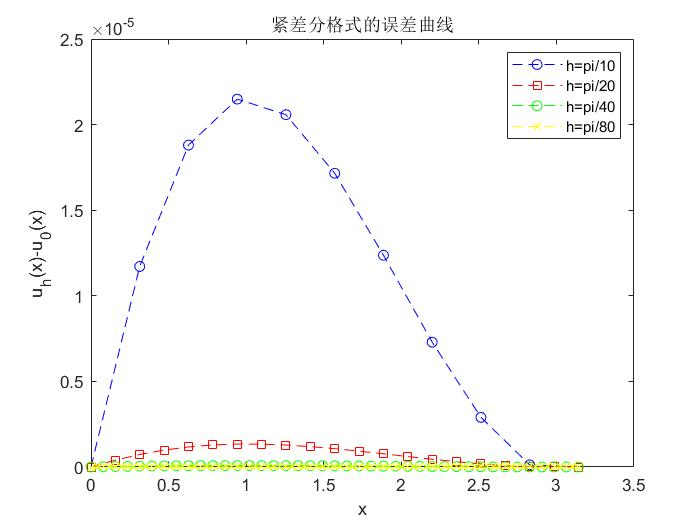
\includegraphics[width=0.7\linewidth]{figures/wucha}
		\caption{紧差分格式不同步长下的误差}
		\label{fig:wucha}
	\end{figure}
\end{document}